\clearpage
\section{Appendix II: Important Figures and Experimental Spectra}
Exp 1401: Observe C7 by GRAPE as the reference. NS=10.\\
Exp 1402: Observe C2 by GRAPE as the reference. NS=10. \\

\begin{figure}[htb]
\begin{center}
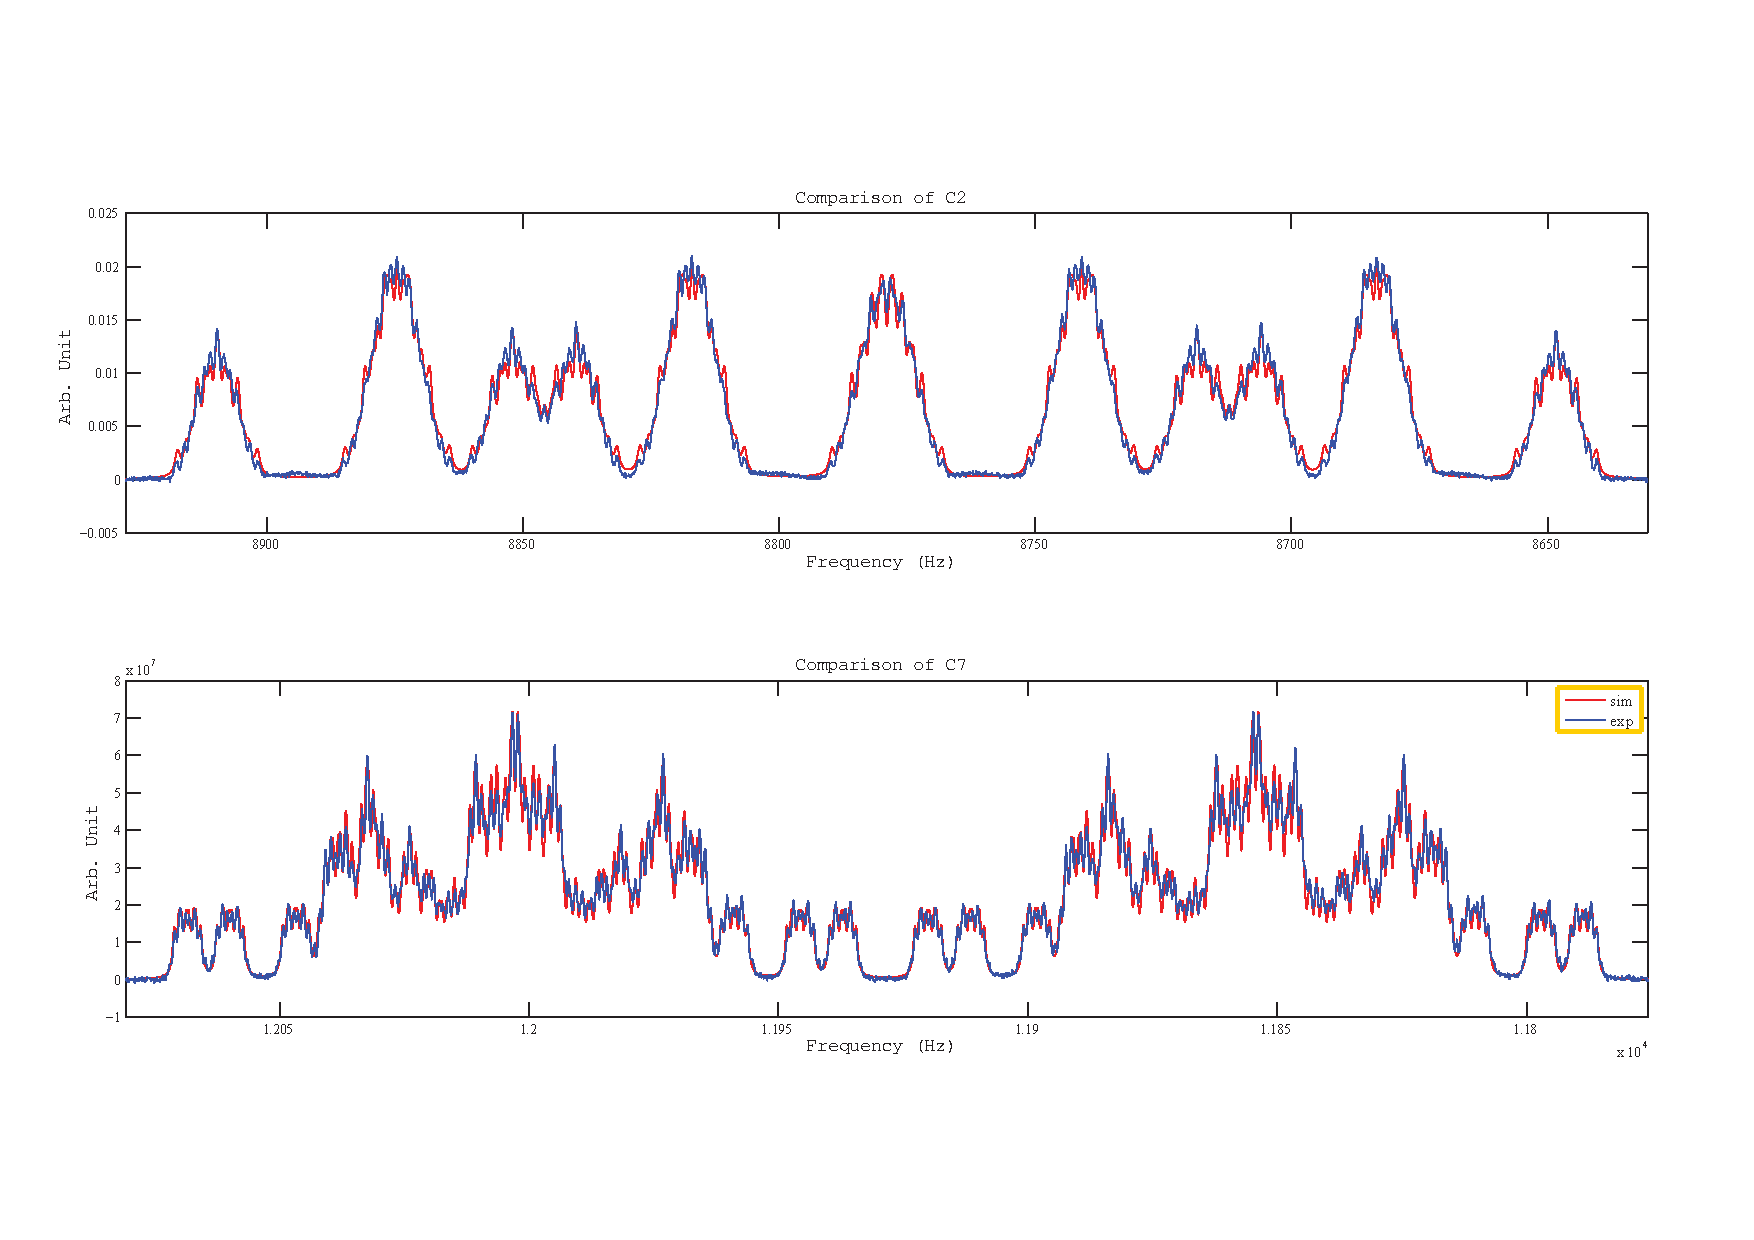
\includegraphics[width=\columnwidth]{Thermal_C2andC7.pdf}
\end{center}
\setlength{\abovecaptionskip}{-0.35cm}
\caption{\footnotesize{Comparison of the thermal for C2 and C7. Blue is experiment and Red is the simulation by the fitted Hamiltonian.}}\label{1401and1402}
\end{figure}

\clearpage
Exp 1403: Observe C7 after encoding1. NS=10.\\
Exp 1404: Observe C2 after encoding1. NS=10.\\

For C2 there is no signal because for Z24567 some couplings are close to 0 and the C2-H couplings broadens the peak. So for 12 qubits, these small couplings cannot be resolved.\\
For C7 it matches well with the simulation. However, the small couplings are annihilated due to the C7-H couplings too.

\begin{figure}[htb]
\begin{center}
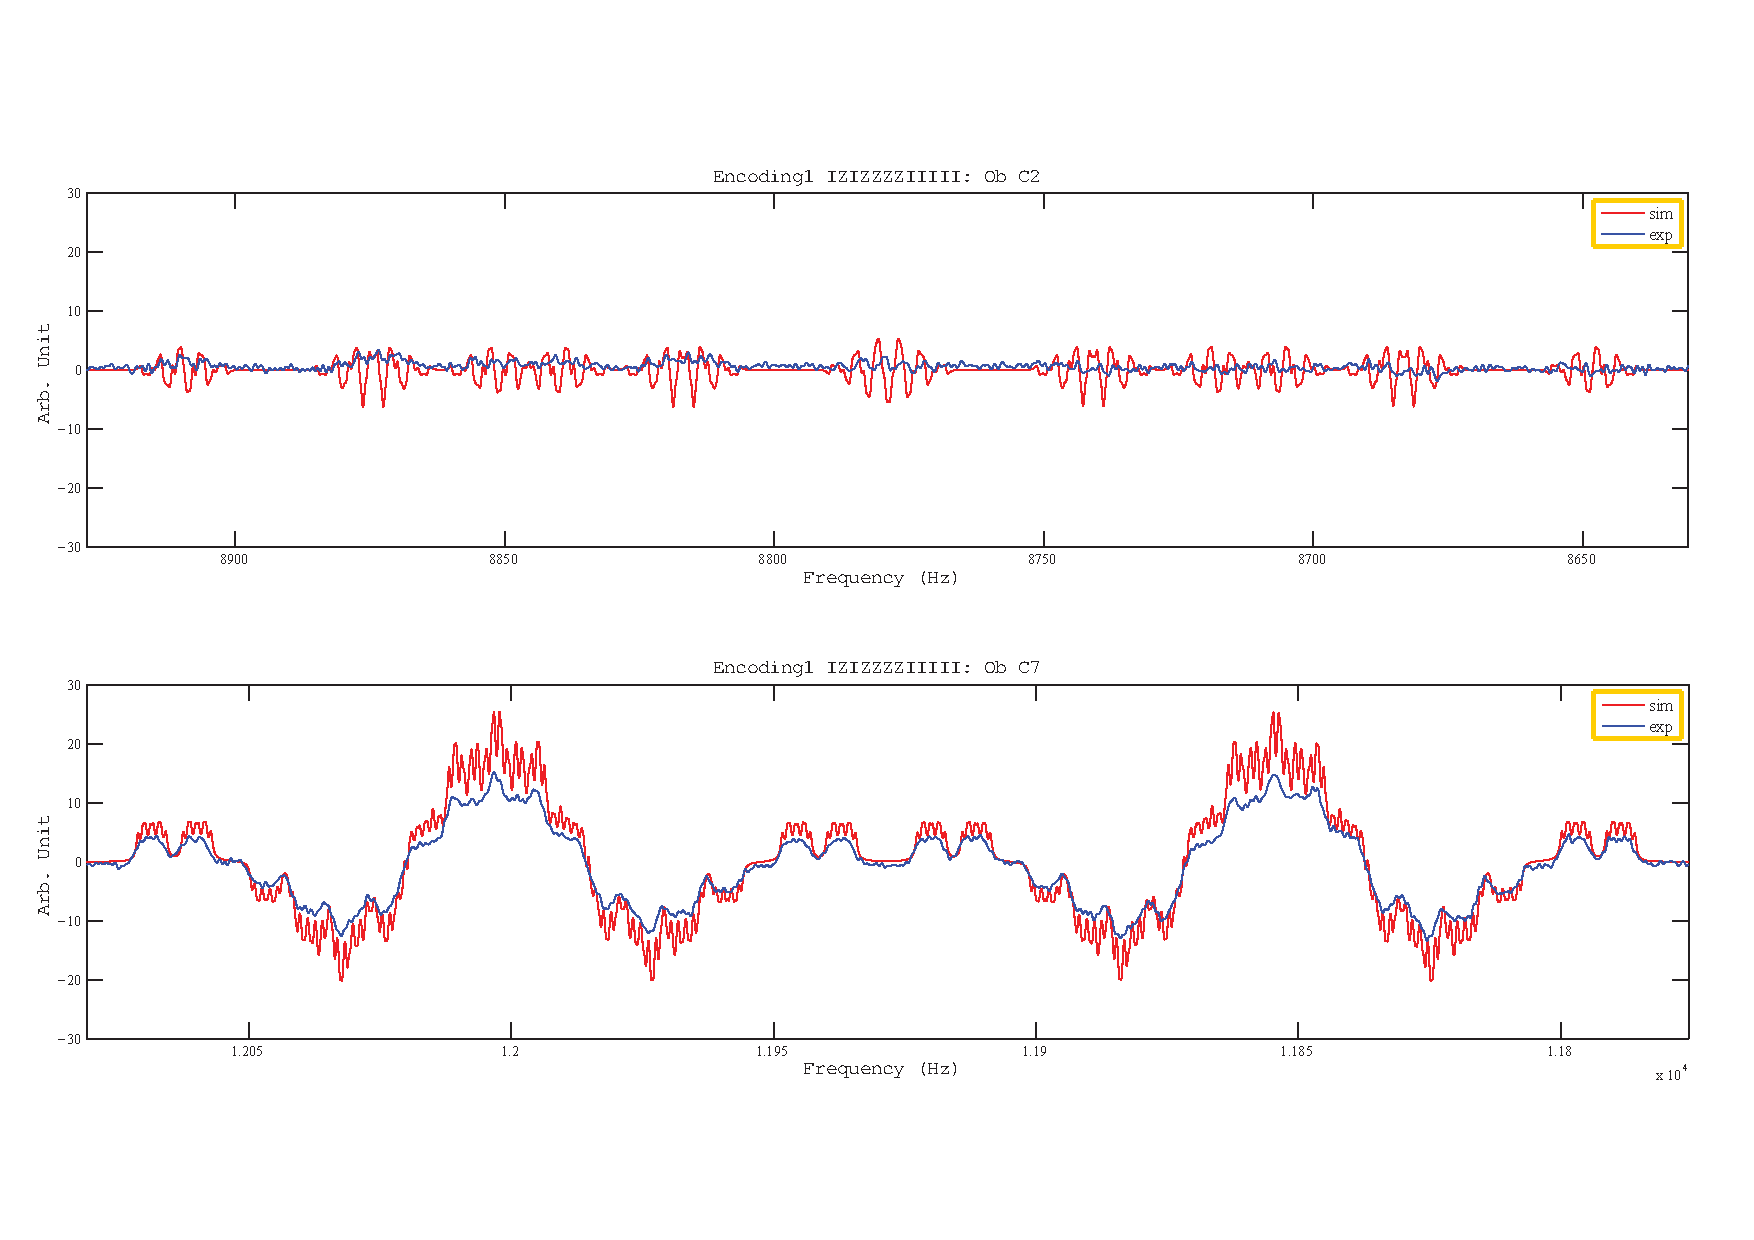
\includegraphics[width=\columnwidth]{Encoding1_without_decouple.pdf}
\end{center}
\setlength{\abovecaptionskip}{-0.35cm}
\caption{\footnotesize{Encoding 1 for C2 and C7 without H decoupled. 10 scans.}}\label{1403and1404}
\end{figure}

\clearpage
Exp 1405: Observe C7 after encoding1 and decouple H. NS=1.\\
Exp 1406: Observe C2 after encoding1 and decouple H. NS=1.\\
\textbf{Note compare with undecoupled experiments, for decoupling experiments I just used 1 scan.}

For C2 the signal is quite close to the 7-qubit case. Good.\\
For C7 the same.

\begin{figure}[htb]
\begin{center}
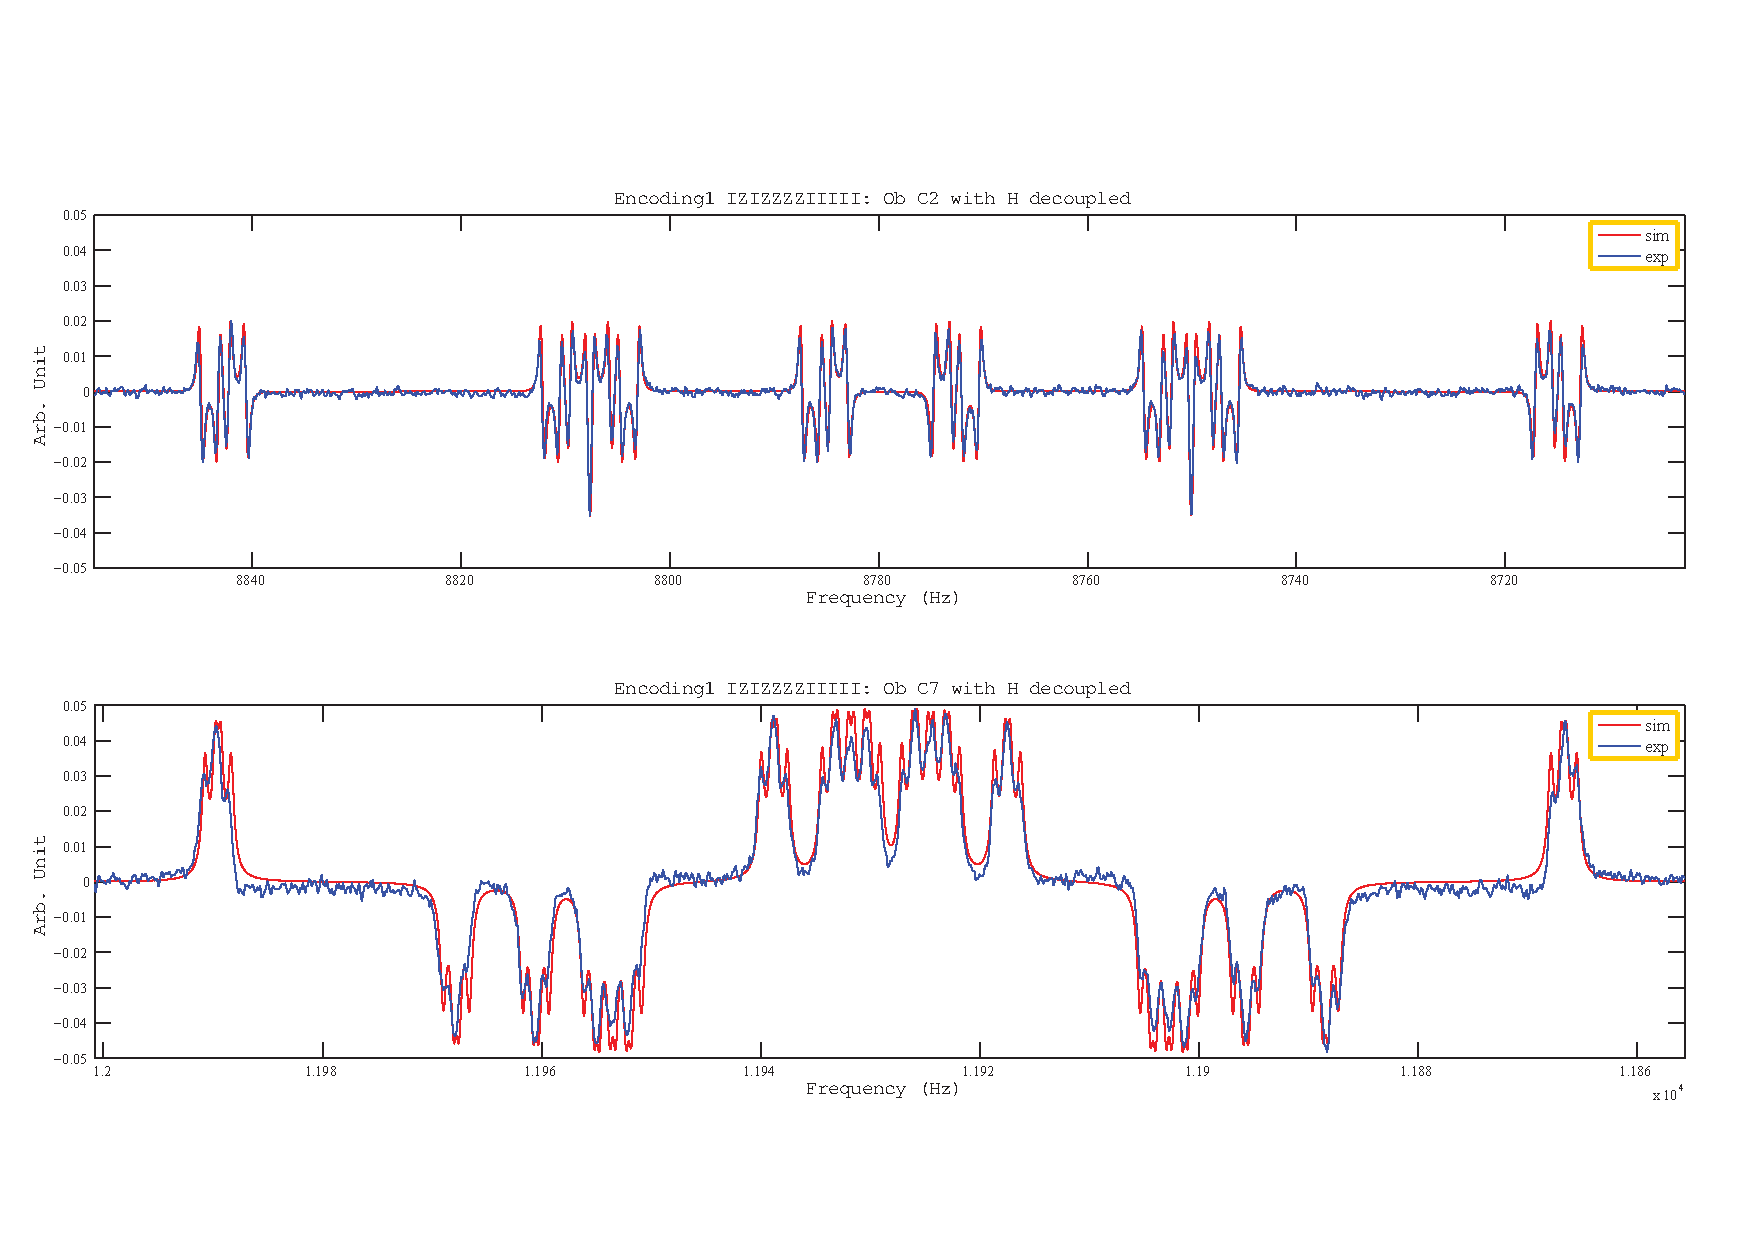
\includegraphics[width=\columnwidth]{Encoding1_with_decouple.pdf}
\end{center}
\setlength{\abovecaptionskip}{-0.35cm}
\caption{\footnotesize{Encoding 1 for C2 and C7 with H decoupled. 1 scan.}}\label{1405and1406}
\end{figure}

\clearpage
Exp 1407: Observe C7 after encoding2. NS=10.\\
Exp 1408: Observe C2 after encoding2. NS=10.\\

For C2 and C7 there are no signals due to the broaden of the C-H couplings.

\begin{figure}[htb]
\begin{center}
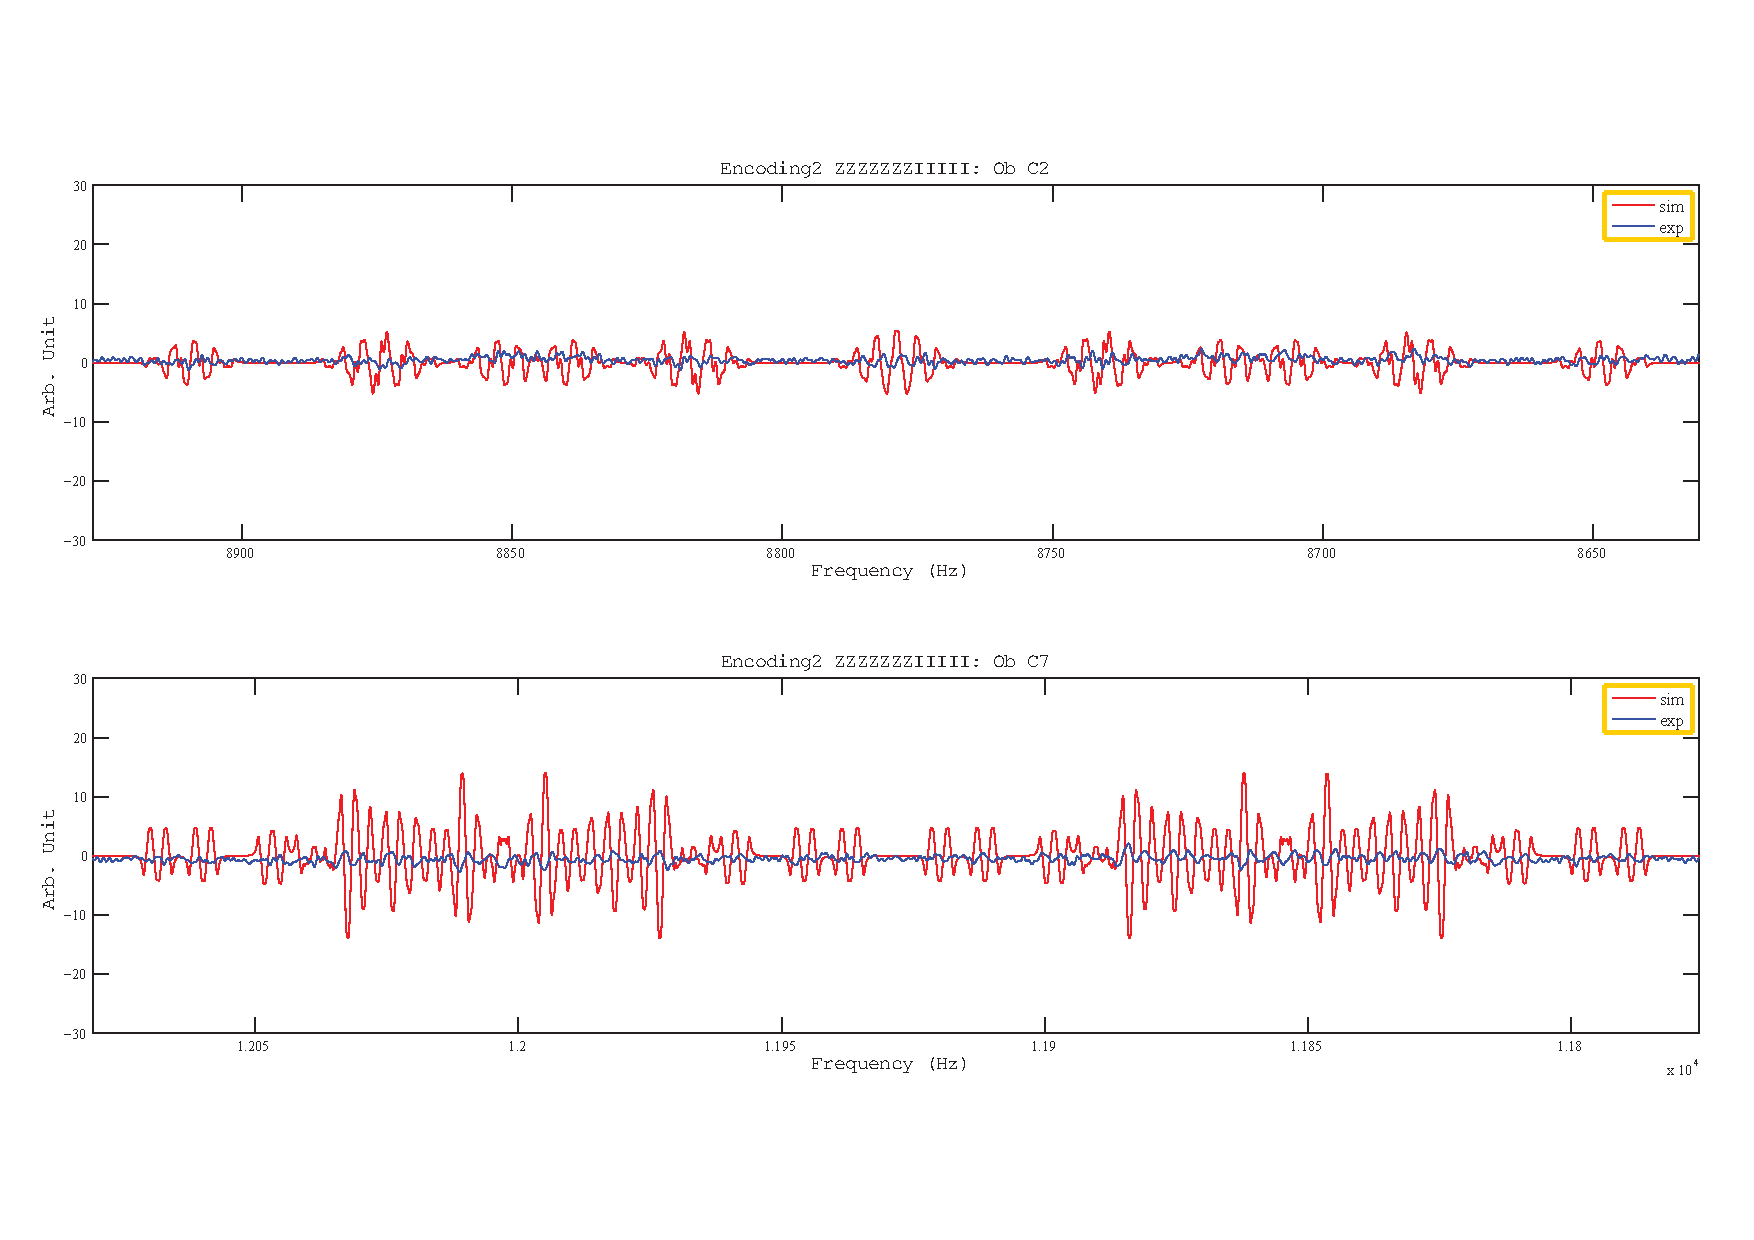
\includegraphics[width=\columnwidth]{Encoding2_without_decouple.pdf}
\end{center}
\setlength{\abovecaptionskip}{-0.35cm}
\caption{\footnotesize{Encoding 2 for C2 and C7 without H decoupled. 10 scans.}}\label{1407and1408}
\end{figure}

\clearpage
Exp 1409: Observe C7 after encoding2 and decouple H. NS=1.\\
Exp 1410: Observe C2 after encoding2 and decouple H. NS=1.\\
\textbf{Note compare with undecoupled experiments, for decoupling experiments I just used 1 scan.}

For C2 and C7 they both look nice.

\begin{figure}[htb]
\begin{center}
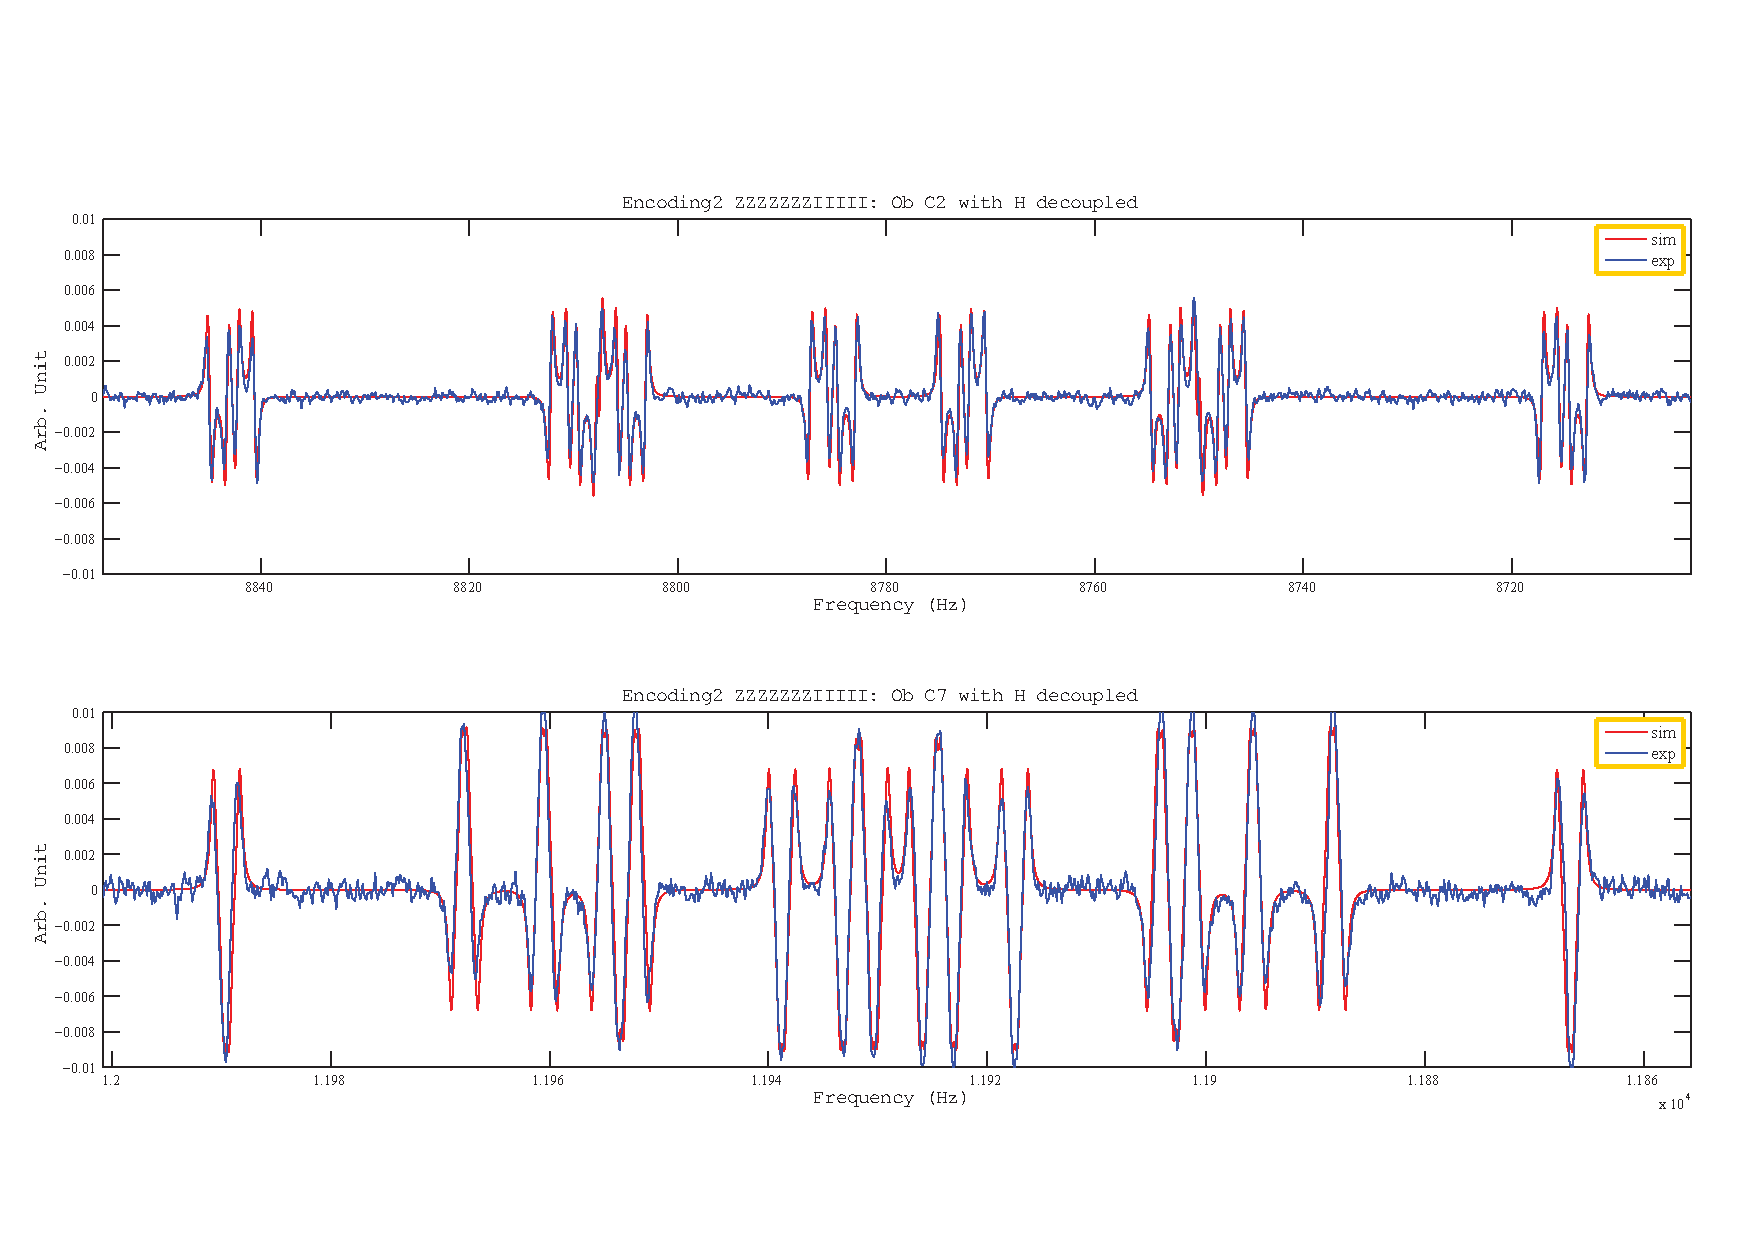
\includegraphics[width=\columnwidth]{Encoding2_with_decouple.pdf}
\end{center}
\setlength{\abovecaptionskip}{-0.35cm}
\caption{\footnotesize{Encoding 2 for C2 and C7 with H decoupled. 1 scan.}}\label{1409and1410}
\end{figure}